%%%%%%%%%%%%%%%%%%%%%%%%%%%%%%%%%%%%%%%%%%%%%%%%%%%%%%%%%%%%%%%%%%%


\documentclass[runningheads,a4paper]{llncs}
\usepackage{graphicx}
\usepackage{amssymb}
\usepackage{amsmath}
\setcounter{tocdepth}{3}
\usepackage{graphicx}
\usepackage{clrscode}
\usepackage{url}



\usepackage{color}


\definecolor{red}{rgb}{1.0,0.0,0.0}
\definecolor{blue}{rgb}{0.0,0.0,1.0}
\definecolor{purple}{rgb}{0.5,0.0,0.5}


\newcommand{\comments}[1]{}
\newcommand{\xj}[1]{\textcolor{red}{(xuejin:#1)}}
\newcommand{\xjmd}[1]{\textcolor{purple}{#1}}



\newcommand{\keywords}[1]{\par\addvspace\baselineskip
\noindent\keywordname\enspace\ignorespaces#1}
\makeatletter
    \newcommand\fcaption{\def\@captype{figure}\caption}
\makeatother
\begin{document}

\mainmatter
\title{Fusing Human Faces}
\author{Xianxiang Wang, and Xuejin Chen}
\institute{University of Science and Technology of China, 230031 Hefei, China\\
\url{kowo@mail.ustc.edu.cn}, \url{xjchen99@ustc.edu.cn}}
\toctitle{Lecture Notes in Computer Science}
\tocauthor{Authors' Instructions}
\maketitle


\begin{abstract}
Face fusion technology grows more important nowadays. In this paper, we introduce a new method that naturally fuses features of the source face into the target face. 
% and target face would still looks natural with its background. 
Our method consists of two steps. 
%
First, the two faces are aligned according to facial landmarks, which provides size, location and distribution of face features. 
Segmenting two faces into several triangles using Delaunay triangulation, warping the corresponding triangle mesh of the two faces into the same shape. 
\xj{What is the relation between the Delaunay triangulations with face features?}
%
Second, \xjmd{we reconstruct a new face using a Poisson reconstruction by fusing the gradient fields of the two faces.} \xj{So what is new in your method?}. 
%
We provide three ways to reconstruct the gradient field.
First, composing a new gradient field by linearly combining gradients of the two input faces.
Second, preserving the larger gradient of each pixel of the two faces.
Third, constructing a new gradient field by preserving the weaker gradient which is proposed by us. \xj{How do you provide the gradient? the weaker gradient comparing with what?}
\xj{I did not see any novelty from your abstract.}


\keywords{Face fusion, facial landmarks, Delaunay triangulation, seamless cloning}
\end{abstract}


\section{Introduction}
These years, there is a great need for face editing application. 
Someone would wonder what would they look like if they have some face features from pop stars.
They may make their faces sharper through face editing applications. While some other people want to know what would they look like when they grow older. these tasks could be accomplished by face fusion. 
%
Progeny appearance prediction is a popular task lately, what if the son of a young couple looks like when he grows up, it is attracting for many people, and this could also be accomplished by face fusion technology.

\xj{Introduce the background or related techniques here. Then discuss the challenges. Why previous does not work. What is the new problem here. }


As we know, different faces have various features.
Someone has a shaper face while the shape of other faces are closer to square. 
There are many ways to build correspondence of two faces. 
\xj{Why do you talk about correspondences after different face features?}
%
In early years, hand marked features of faces are used to build correspondence of two faces \cite{fbim}, because of the lack of automatic face feature detection techniques.
There are a lot of labour work needed. 
Most people do not want to mark the features manually. 
Lately, a five-feature points based face fusion method \cite{mhf} was proposed.
Five feature points are detected automatically, which could save a lot of time for users.
Then with these feature points, two faces could be warped and fused into one. 
In fact, five feature points are not enough to represent a face.
When we use the sparse correspondence to generate a new face, the result is weird.

Given two faces, the face we want to extract its features and fuse its features into the other face named source face, the face which keeps its background and let source face features fuse into self named target face. 
There are 68 facial landmarks are detected by using an Ensemble of Regression Trees \cite{fld} in our method, thus we know exactly the features and size of the face. 
Facial landmarks indicate the face structures, in other words, the distribution of face features, while the face gradients indicate the face details. When we fuse two faces, first, we warp two faces to make sure the structures of two faces are the same. Second, we fuse the gradients of two faces, in order to maintain the main features of the source face and illumination information of the target face, we reconstruct the gradients for new face by keeping the larger gradients of the source face and part of lower gradients of the target face, then, we could recover the fused face by seamless cloning \cite{pie}.

\section{Related work}
In this section, we summarize existing approaches that are related to our work.

\textbf{Face Morphing.} Face morphing is commonly referred as the animated transformation of one digital face image to the other, in most case, the background of the face image is pure in order to make us focus on transition of the face itself.
%
 Beier and Neely \cite{fbim} developed a user interface to build correspondences of two faces by a group of line pairs. However, this procedure is tedious and time-consuming.
 Besides, hand-marked features are not precise.
 After building correspondences, the corresponding pixels are linearly interpolated.  Wolberg \cite{wol} proposed a mesh-based method to build correspondences of two faces, the correspondences of two faces are referred as meshes instead of line pairs. Karungaru et al. \cite{mhf} detect five feature points as control points, then segment face images into several triangles according to control points, next warp the face images according to corresponding triangles. 
 These face morphing methods have a different way in building correspondences.
 Their aim is creating a seamless transition from one face to the other.
 \xj{Not only talk about the correspondences here. The key point is how different of the morphing technique and your method. Based on my understanding, you also require a correspondence extraction step. So what is the difference? }

\textbf{Face Swapping.} Face swapping is also known as face replacement, means transferring a face from a source photo onto a face appearing in a target photo in order to generate a new genuine face.
\xj{You solve the same problem, right? If not, discuss the main difference. }
%
The most early work for face swapping is \cite{exchface}, but the results are not that realistic. 
Later, the results are better \cite{de1}\cite{de2}\cite{de3}\cite{de4} and mainly used for deidentification. \xj{What is deidentificaation?}
The main problem for face swapping is pose variation, most works solve this problem by using 3D models \cite{de3}\cite{3d1}\cite{onseg}. Nirkin et al. \cite{onseg} transfer the face from the source image onto the target image using a 3D face model, they first detect facial landmarks used to establish 3D pose and facial expression for 3D face shape, then use a FCN to segment the visible parts of faces from their context and occlusions, at last, source face is blended-in with the target context using image seamless cloning \cite{pie}.
This step would fail when blending very different facial hues.
\xj{what is different in your method?}
 Korshunova et al. \cite{faceswapping} propose a network to generate a source face that could replace the face in target image.
 One network could only generate faces of the same type, for example, a net named CageNet could only generate the face of Nicolas Cage. 
 Those two methods mentioned above may greatly change the lightning condition of the face on the target image because they just transfer the source face onto the target image, but not containing any information of the target face. 
 Bitouk et al. present a system for automatic  face replacement in images, given a target face image, the system would retrieve a face with similar pose, lightning and color condition, then use such a face to replace the face on the target image, the limitation of the source face is clear, it must have a similar pose and lightning condition with the target face. 
 %
 The main difference between face swapping and our task is that we want keep some features of the target face but not to replace the target face with the source face, how to fuse the features of the source faces into the target faces is our main consideration.
 \xj{So face morphing problem is similar because both of you and face morphing should keep the features of two faces. }



\section{Fusing features of the source face into the target face }
\xj{Do not use such a long sentence for a section title!}


\section{Face fusion}
\label{sec:facefusion}

Our task is to fuse face features of a source face into a target face.
\xjmd{Our method consists of two steps: face alignment and face feature fusion, as shown in Fig.~\ref{fig:pipeline}. }
%
First, aligning two faces, it is necessary to calculate the location and the size of the facial part from each face image. 
With the help of facial landmarks \cite{fld}, it is quick to do so. 
But only knowing the location and size of two faces is not enough, we need to know where are the eyes, nose and other parts of the face, different faces have different face features, some people have a big nose while others with a small one, some people's nose is closer to eyes while others' nose is farther to eyes. Still, with the help of facial landmarks, we know exactly the distribution of the face features.
%
Second, by aligning two faces, we know the parts on one face and its corresponding parts on the other face. Then, we could fuse features of one face into other face from part to part.

\begin{figure}
	\centering
    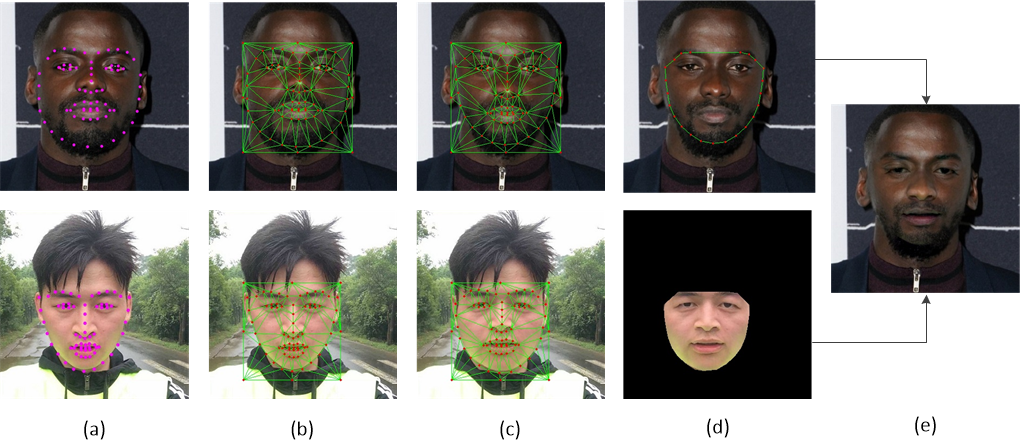
\includegraphics[width=4.8in]{images/pipeline.png}
    \caption{Pipeline of our work: (a) Perform facial landmark detection on two faces. (b) Triangulate two faces according to the facial landmarks. (c) Calculate new facial landmarks by interpolating two groups of facial landmarks, warp two faces according to the new facial landmarks. (d) Reconstruct gradients on facial part for fused face . (e) Fuse features of source face into target face by seamless cloning.}
    \label{fig:pipeline}
\end{figure}

\subsection{Face alignment}
There are many ways to find facial landmarks \cite{fld2}\cite{fld3}\cite{fld4}\cite{fld}, we adopt \cite{fld}, \xj{because of what?}.
It is implemented in Dlib.

In Fig. 1(a), with the landmarks of two faces, two faces' bounding box could be calculated.
A%s we talked before, different faces have different facial landmarks, so the source face's bounding box and the target face's bounding box could have different ratio of height and width. 
In order to align two faces easily, we reshape the bounding boxes of two faces into square by stretching the shorter side of the bounding box, and we will get a bounding square of face. Then, we need to enlarge the bounding squares of two face a little for the consensus of triangulation of two faces as shown in Fig.~\ref{fig:pipeline}(b). 
%
The center point and side length of bounding square of source face are denoted as $\mathbf{c}_s$ and $l_s$, the center point and side length of bounding square of target face are denoted as $\mathbf{c}_t$ and $l_t$. The index of facial landmarks $i \in \{1...N\}$, $N$ is the number of facial landmarks, for each point $\mathbf{p}_i$ inside the bounding square of source face, we could calculate its corresponding location on the target face by following mapping function:
%
\begin{equation} \label{eq:mapping}
f(\mathbf{p}_i)=\frac{l_t}{l_s}(\mathbf{p}_i-\mathbf{c}_s)  + \mathbf{c}_t
\end{equation}
%
Before we triangulate a face according to facial landmarks, we need make sure that the transition from the background to the face is natural, so we add some points into the facial landmarks to help triangulate the faces, these points are four corners of bounding squares and four midpoints on four sides of bounding squares. The facial landmarks we need to triangulate on the source face and the target face are denoted as $F_{s}$(the red points on the face image in second row of Fig. 1(b)) and $F_{t}$(the red points on the face image in first row of Fig. 1(b)) respectively. The facial landmarks that we want could be calculated by interpolating $F_s$ and $F_t$ and are denoted as $F_n$, with these new facial landmarks, we could create a new face structure. for each point in $F_s$, $F_t$ and $F_n$, they are denoted as $F_{s_i}$, $F_{t_i}$ and $F_{n_i}$ respectively.
$$F_{n_i} = \alpha \cdot f(F_{s_i})+(1-\alpha)\cdot F_{t_i} \eqno{(2)}$$
$\alpha$ controls which face structure we prefer more, if $\alpha$ is small, the new face structure would look more like the target face, in other words, the profile of the new face and the distribution of the new face features would look more like the target face.

After triangulating two faces according to $F_s$ and $F_t$ using Delaunay Triangulation, we get two groups triangles from the source face and the target face, denoted as $T_s$ and $T_t$ respectively. 
The two faces corresponding triangles are not of the same shape because of different facial landmarks. 
what we need to do is to make sure the shape of corresponding triangles of two faces are the same. we could get $T_n$ by triangulating $F_n$. Warping $T_{t}$ to the $T_{n}$, and warping $T_s$ in a similar way. In Fig. 1(c), the source face and the target face are warped, the size and the location of their bounding squares are different at each face image, but the shape of the corresponding triangles of two faces  are the same.
\xj{Use uppercase letters for the first letter in each sentence.} 


\subsection{Face fusion}
After warping two faces, we have two faces of the same structures and the same distribution of face features, but the size and the location of their bounding square are different, we extract the bounding square area of the source face, scale and translate this area to the same size and location of the bounding square of the target face, the new source face image is shown in Fig. 2(b).

As we can see from the Fig. 2, the triangles of the source face and the target face are exactly at the same location and of the same shape and size. the purpose of our task is to fuse the source face features into the target face, so we need to know the profile of the source face, then extract the facial part from the source face image. In Fig. 2(c), the yellow outline is generated from the facial landmarks, but we need to shrink the profile a little to make sure that all the pixels are from the face, inside the blue outline is $\Omega$, $\Omega$ stands for the facial part we are going to fuse.

\begin{center}
    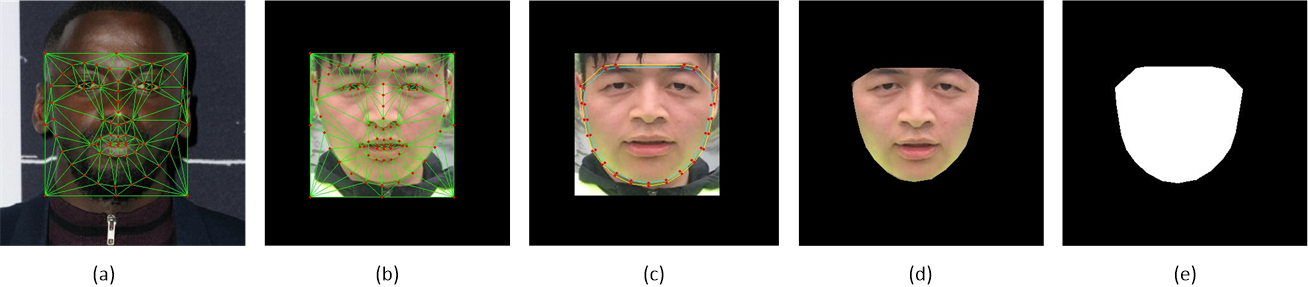
\includegraphics[width=4.8in]{images/extract.png}
    \fcaption{(a) The target face warped according to $F_n$. (b) The warped source face after being translated and scaled. (c) Yellow outline is generated from the landmarks of the warped source face, light blue outline is shrank a little from the yellow profile. (d) Facial part of the warped source face that inside $\Omega$. (e) Facial mask.}
\end{center}

The target face and the source face are shown in Fig. 2(a) and 2(b), we fuse the gradients of of two faces, recover the face from the fused gradients by seamless cloning.

The gradient of the source face is denoted as $g_s$, the gradient of target face is denoted as $g_t$, $g$ is the gradient we will use to recover the face, there are three ways we tried to fuse the gradients of two faces.

For the first way, The guidance field $g$ could be generated  by linearly combining $g_s$ and $g_t$:

$$g = \beta \cdot g_s+(1-\beta) \cdot g_t \eqno{(3)}$$

For the second way, at each point in $\Omega$, retain the stronger gradients in $g_s$ or in $g_t$:

$$
for\ all\ x \in \Omega\text{, } g(x)=\left\{
\begin{aligned}
g_s(x) &&{if |g_s(x)|>|g_t(x)|}\\
g_t(x) &&{else}\\
\end{aligned}
\right.
\eqno{(4)}$$

For the third way, define $g$ by linearly combination of $g_d$ and $g_t$:

$$g = \beta \cdot g_d+(1-\beta) \cdot g_t \eqno{(5)}$$

The definition of $g_d$ is:

$$ for\ all\ x \in \Omega\text{, } g_d(x)=\left\{
\begin{aligned}
g_t(x) &&{if \ |g_s(x)|< \theta_1 \ or \ |g_t(x)|< \theta_2}\\
g_s(x) &&{else}\\
\end{aligned}
\right.
\eqno{(6)}$$

$g_d$ contains the bigger gradients of the $g_s$ and lower gradients of $g_t$, if $g_s(x)$ is smaller than the threshold $\theta_1$ and $g_t(x)$ is smaller than the threshold $\theta_2$, then $g_d(x)$ keeps the gradient from $g_t$ at point $x$, so it contains main features of the source face and the part of the lightning condition of the target face. Fig. 3(a) and Fig. 3(b) are facial parts of the target face and source face, they share the same profile and distribution of features, Fig. 3(c) shows that which parts of $g_d$ are come from $g_t$ or $g_s$, for all $x \in \Omega$ and for each channel, if $g_d(x)$ is come from $g_s(x)$, then the corresponding part in Fig. 3(c) is brighter. \\
Finally, we could use $g$ to recover the face we want on the target face image by seamless cloning, we could control how much features from the source face to fuse into target face by using the first way or the third way.


\xj{All these gradient fusion methods were introduce in Poisson image editing paper. No new technique here. }
\begin{center}
    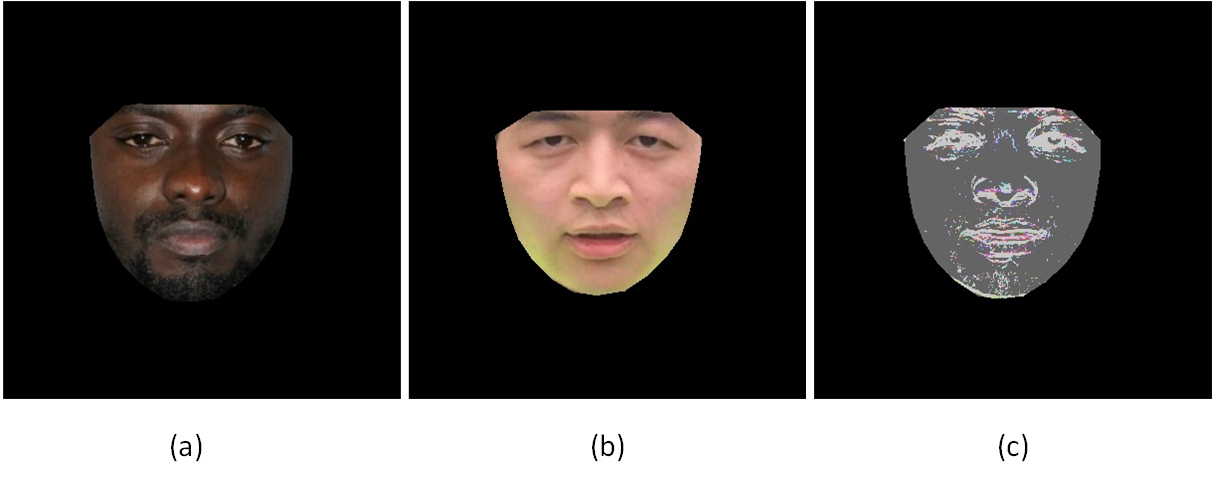
\includegraphics[width=4.8in]{images/labelmask.png}
    \fcaption{(a) Facial part of target face. (b) Facial part of the source face. (c) A mask indicate which part of $g_d$ are come from $g_s$ or $g_t$. \xj{what does the color in (c) mean? If you want to show where the gradient comes from, it should be a binary mask. If you want to show the weight, it should be a gray weight map. But here is a color map...}}
\end{center}

\section{Experiments}

\subsection{Comparison of different gradient reconstruction}
\begin{center}
    \includegraphics[width=4.8in]{images/3cmp.png}
    \fcaption{The effects of different gradient reconstruction: (a) Source face image. (b) Target face image. (c) Fusing face by linearly combining the gradients of two faces. (d) Fusing face by keeping the larger gradients of two faces. (e) Fusing face through weaker gradient preserving method.}
\end{center}

Fig. 4 shows the effects of different face gradient reconstruction. From Fig. 4(c), we can see that direct linear combination of two faces gradients could bring too much illumination from source face into target face, which makes face looks very unnatural. If we kept the larger gradients of two faces, the illumination of the target face would be strongly broken, more importantly, we can't control how much features we are going to fuse from source face into target face. In Fig. 4(e), the lightning condition and facial hues is closest to the target face image, when we reconstruct gradients using the third method, we only keep the larger gradients of the source face which means the main features of the source are preserved, and we keep lots of the weaker gradients of the target face, which means we maintain some illumination information and facial hues of the target face.

\xj{Since you cut the background out in your fusion step, it is similar with a morphing problem. Compare your method with face morphing techniques. }
\subsection{How the different parameters effect face fusion}
In this paper, there are four parameters we can control, they are $\alpha$, $\beta$, $\theta_1$, $\theta_2$. $\alpha$ controls the structure of human faces, in other words, it controls the profile and the distribution of features of human faces. $\beta$ controls the details of human faces, like wrinkles and textures. With $\alpha$ and $\beta$, we can control how much content we want to fuse from source face into target face. If the gradients of source face is weaker than $\theta_1$ and the gradients of target face is weaker than $\theta_2$, then we retain the gradients of the target face, otherwise we keep the gradients of the source face.\\
Fig. 5 shows how $\alpha$ effects the fused results, $\beta = 0.5$, $\theta_1 = 10$, $\theta_2 = 15$. As the $\alpha$ grows bigger, the distribution of face features of fused face is more like the source face.

\begin{center}
    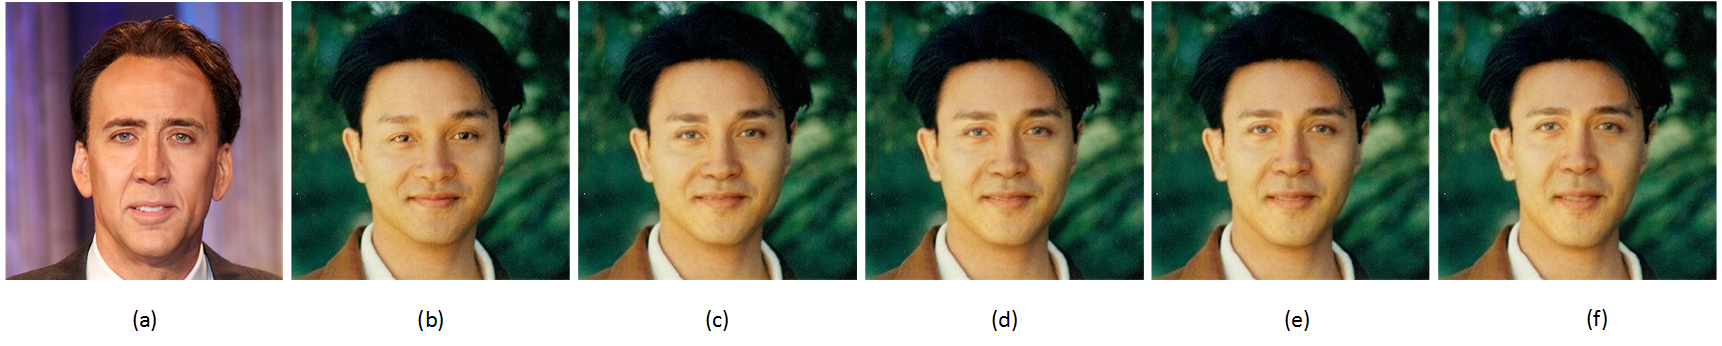
\includegraphics[width=4.8in]{images/pro.png}
    \fcaption{(a) Source face. (b) Target face. (c) Fused face, $\alpha = 0.2$. (d) Fused face, $\alpha = 0.4$. (e) Fused face, $\alpha = 0.6$. (f) Fused face, $\alpha = 0.8$.}
\end{center}

Fig. 6 shows how $\beta$ effects the fused result, $\alpha = 0.5$, $\theta_1 = 10$, $\theta_2 = 15$. As the $\beta$ grows bigger, the fused result has more details from source face.

\begin{center}
    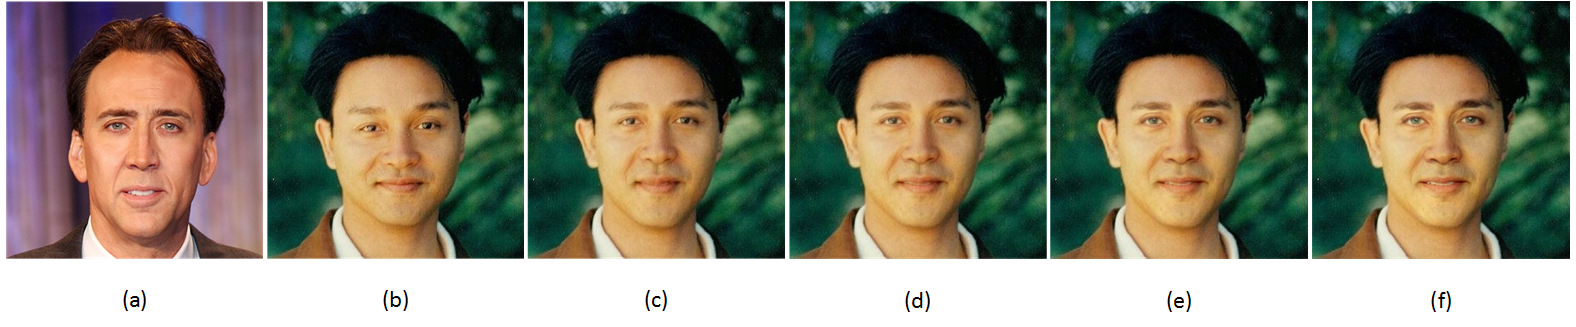
\includegraphics[width=4.8in]{images/detail.png}
    \fcaption{(a) Source face. (b) Target face. (c) Fused face, $\beta = 0.2$. (d) Fused face, $\beta = 0.4$. (e) Fused face, $\beta = 0.6$. (f) Fused face, $\beta = 0.8$.}
\end{center}

If we want to only keep main features of source face, we could only retain stronger gradients of the source face, Fig. 7 shows that the fused results are more natural as more weaker gradients of the source face are been dropped. $\alpha = 0.5$, $\beta = 0.5$, $\theta_2 = 40$. The weaker gradients carry too much illumination information and facial hues of the source face, when these gradients are brought into the fused results, the results are become very unnatural.

\begin{center}
    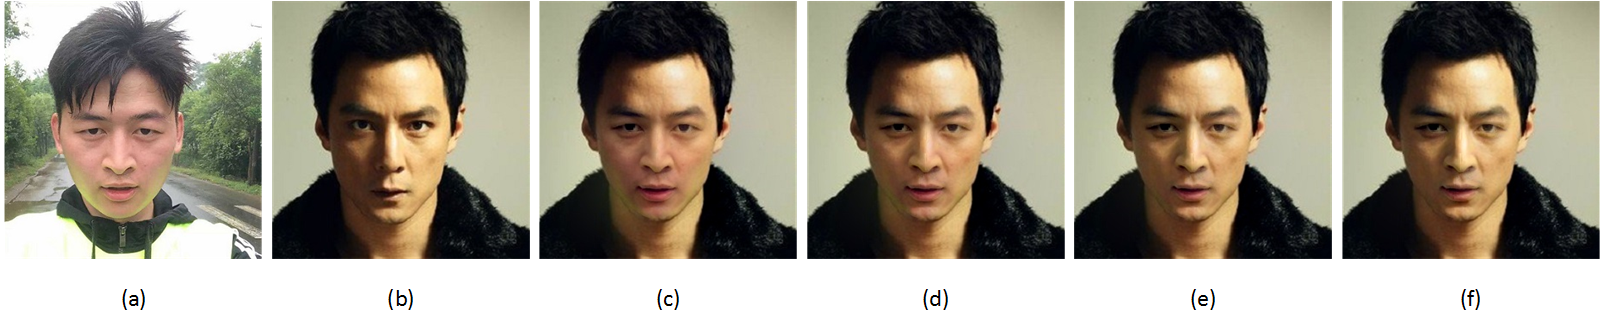
\includegraphics[width=4.8in]{images/thd1.png}
    \fcaption{(a) Source face. (b) Target face. (c) Fused face, $\theta_1 = 2$. (d) Fused face, $\theta_1 = 4$. (e) Fused face, $\theta_1 = 6$. (f) Fused face, $\theta_1 = 8$.}
\end{center}

When we fuse the main features of source face into target face, somehow, we need to erase the main features of target face. In fact, we want to keep the illumination information of the target face, both the weaker gradients of source face and weaker gradients of target face are being kept. For Fig. 8, it shows the experiment on $\theta_2$,  $\alpha = 0.5$, $\beta = 0.5$, $\theta_1 = 10$, when the $\theta_2$ grows bigger, more stronger gradients are preserved, as we could see, more shadows are preserved.

\begin{center}
    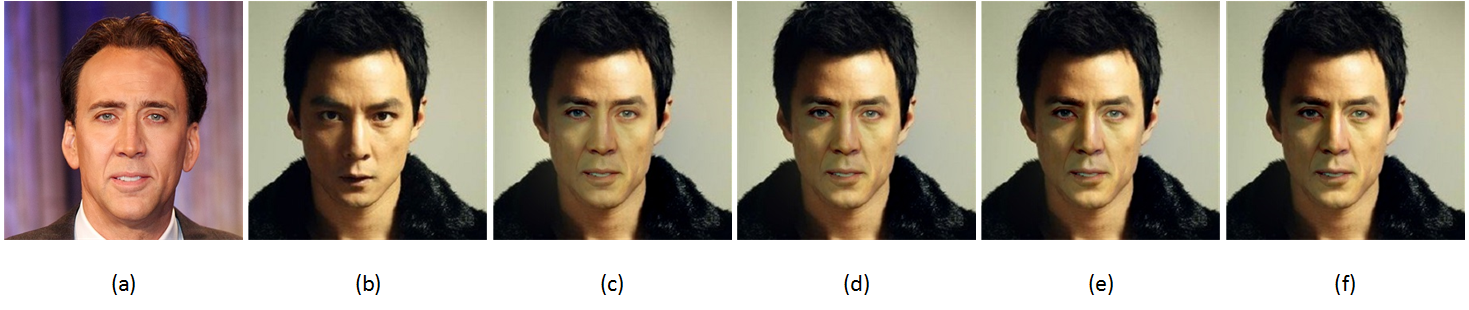
\includegraphics[width=4.8in]{images/thd2.png}
    \fcaption{(a) Source face. (b) Target face. (c) Fused face, $\theta_2 = 10$. (d) Fused face, $\theta_2 = 20$. (e) Fused face, $\theta_2 = 30$. (f) Fused face, $\theta_2 = 40$.}
\end{center}

Although our work are not aiming at face swapping task, we still could create similar effects by setting $\beta = 1$, this means we almost preserving all the gradients of source faces, but only keep part of weaker gradients of target faces. We compare our results and the work of Korshunova et al. \cite{faceswapping}, in Fig. 9, the source face of all the results is from Fig. 8(a), we can see that our results keep more illumination information and facial hues of target faces which makes our results more natural, but in Fig. 9(c), our result fail to catch the lightning condition of the target face from a high level, this is where we need improve.

\xj{compare with FaceSwap \cite{autorep}.}

\begin{center}
    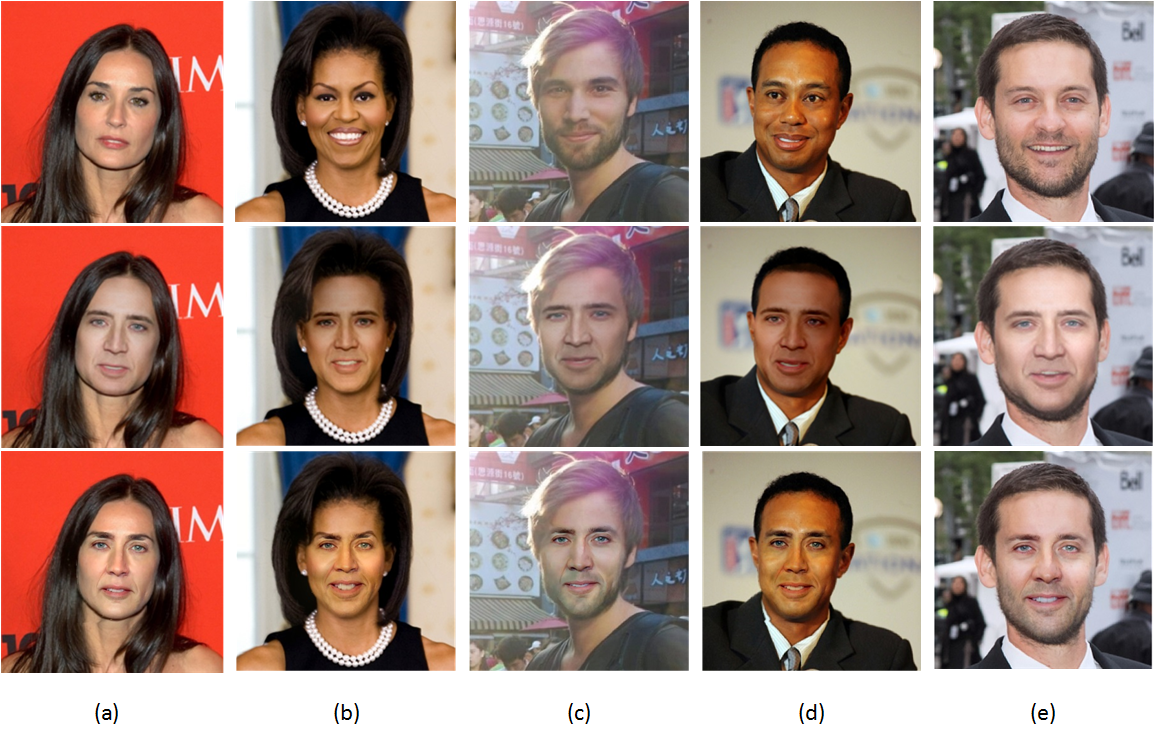
\includegraphics[width=4.8in]{images/vs.png}
    \fcaption{The first row are the original target face, the second row are the results of Korshunova et al., the third row are our results.}
\end{center}

\section{Conclusions}

We developed a face fusion method that could automatically fusing one face features into the other face. When we are considering fusing human faces, there are two parts we are going to fuse, one is face structures, the other is face details. The 68 facial landmarks are enough to align two faces precisely. The illumination of the source face might pollute the target face, but the method we proposed preserves as much illumination information as possible while decreasing the affection of illumination of the source face. At mean time, we developed a user interface for letting users control how much features they want from the source face to fuse into the target face.
\begin{thebibliography}{4}

\bibitem{fbim} Beier, T., Neely, S.: Feature-based image metamorphosis. In: ACM SIGGRAPH Computer Graphics, Vol. 26, No. 2, pp. 35-42 (1992)
\bibitem{wol}Wolberg, G.: Image morphing: a survey. In: The visual computer, 14(8), 360-372 (1998)
\bibitem{pie}P��rez, P., Gangnet, M., Blake, A.: Poisson image editing. In: ACM Transactions on Graphics (TOG), Vol. 22, No. 3, pp. 313-318 (2003)
\bibitem{mhf}Karungaru, S., Fukumi, M., Akamatsu, N.: Morphing Human Faces: Automatic Control Points Selection And Color Transition. In: International Conference on Computational Intelligence, pp. 224-227 (2004)
\bibitem{exchface}Blanz, V., Scherbaum, K., Vetter, T., Seidel, H. P.: Exchanging faces in images. In: Computer Graphics Forum, Vol. 23, No. 3, pp. 669-676 (2004)
\bibitem{autorep}Bitouk, D., Kumar, N., Dhillon, S., Belhumeur, P., Nayar, S. K.: Face swapping: automatically replacing faces in photographs. ACM Transactions on Graphics (TOG), 27(3), 39. (2008)
\bibitem{de1}De La Hunty, M., Asthana, A., Goecke, R.: Linear facial expression transfer with active appearance models. In: International Conference on Pattern Recognition (ICPR) (2010)
\bibitem{de2}Ross, A., Othman, A.: Visual cryptography for biometric privacy. In: IEEE transactions on information forensics and security.(2011)
\bibitem{de3}Lin, Y., Wang, S., Lin, Q., Tang, F.: Face swapping under large pose variations: A 3D model based approach. In: International Conference on Multimedia and Expo (ICME), pp. 333-338 (2012)
\bibitem{3d1}Lin, Y., Lin, Q., Tang, F., Wang, S.: Face replacement with large-pose differences. In: Proceedings of the 20th ACM international conference on Multimedia. (2012)
\bibitem{fld2}Xiong, X., De la Torre, F.: Supervised descent method and its applications to face alignment. In: Proceedings of the IEEE conference on computer vision and pattern recognition.(2013)
\bibitem{fld3}Ren, S., Cao, X., Wei, Y., Sun, J.: Face alignment at 3000 fps via regressing local binary features. In: Proceedings of the IEEE Conference on Computer Vision and Pattern Recognition.(2014).
\bibitem{fld4}Cao, X., Wei, Y., Wen, F., Sun, J.: Face alignment by explicit shape regression. In: International Journal of Computer Vision. (2014)
\bibitem{de4}Mosaddegh, S., Simon, L., Jurie, F.: Photorealistic Face de-Identification by Aggregating Donors�� Face Components. In: Asian Conference on Computer Vision, pp. 159-174 (2014)

\bibitem{fld}Kazemi, V., Sullivan, J.: One millisecond face alignment with an ensemble of regression trees. In: Proc. IEEE Conf. Computer Vision and Pattern Recognition (CVPR), pp. 1867-1874 (2014)

\bibitem{faceswapping}Korshunova, I., Shi, W., Dambre, J., Theis, L.: Fast face-swap using convolutional neural networks. arXiv preprint arXiv:1611.09577. (2016)
\bibitem{onseg}Nirkin, Y., Masi, I., Tran, A. T., Hassner, T., Medioni, G.: On Face Segmentation, Face Swapping, and Face Perception. arXiv preprint arXiv:1704.06729. (2017)


\end{thebibliography}



\end{document}
